\documentclass{standalone}
\usepackage{pgfplots}
\pgfplotsset{compat=1.17} % Set compatibility to avoid warnings
\usepgfplotslibrary{fillbetween} % Load library for 'name path'

\begin{document}

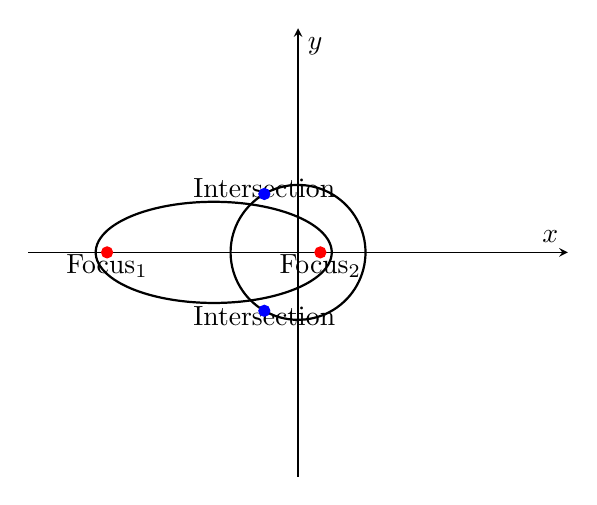
\begin{tikzpicture}
    % Define parameters
    \def\a{1.75}          % Semi-major axis of the ellipse
    \def\b{0.75}          % Semi-minor axis of the ellipse
    \def\centerX{-1.25}   % x-coordinate of the ellipse center
    \def\centerY{0}       % y-coordinate of the ellipse center

    \begin{axis}[
        axis equal,
        axis lines=middle,
        xmin=-4, xmax=4,
        ymin=-3, ymax=3,
        xlabel={$x$},
        ylabel={$y$},
        ticks=none
    ]
        % Draw the unit circle centered at the origin
        \addplot[thick, domain=0:360, samples=100, smooth, name path=circle] 
            ({cos(x)}, {sin(x)});

        % Draw the ellipse using parameters for a, b, and center
        \addplot[thick, domain=0:360, samples=100, smooth, name path=ellipse] 
            ({\centerX + \a*cos(x)}, {\centerY + \b*sin(x)});
        
        % Calculate foci positions based on a and b
        \pgfmathsetmacro{\c}{sqrt(\a^2 - \b^2)}
        
        % Plot points for the foci of the ellipse
        \addplot[only marks, mark=*, mark options={scale=1, color=red}] coordinates 
            {({\centerX - \c}, \centerY) ({\centerX + \c}, \centerY)};
        \node at ({\centerX - \c}, -0.2) {$\mathrm{Focus}_1$};
        \node at ({\centerX + \c}, -0.2) {$\mathrm{Focus}_2$};

        % Add estimated intersection points between the circle and ellipse
        \addplot[only marks, mark=*, mark options={scale=1, color=blue}] coordinates 
            {(-0.5, 0.866) (-0.5, -0.866)};
        \node at (-0.5, 0.95) {Intersection};
        \node at (-0.5, -0.95) {Intersection};

    \end{axis}
\end{tikzpicture}

\end{document}
